\documentclass{article}
\usepackage[margin=1.0in]{geometry}
\usepackage{titling}
\usepackage{graphicx}
\usepackage{float}
\usepackage[T1]{fontenc}

\begin{document}
	
	%%% title
	\setlength{\droptitle}{-5em}
	\title{4.0 Functions}
	\date{10-7-2020}
	\author{}
	\maketitle
	
	%%% first section
	\section{Constant}
	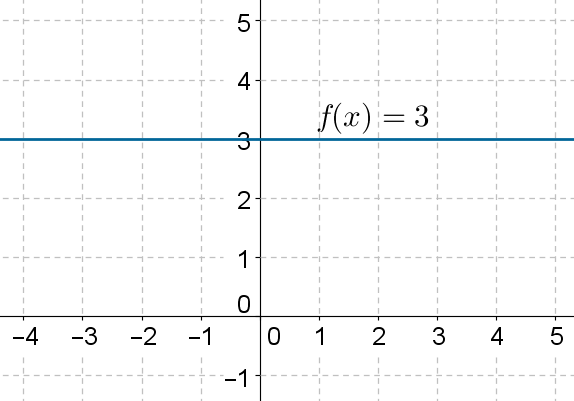
\includegraphics[scale=0.5]{pics/constfunc.png}
	\newline \newline
	Every input returns the same output
	\newline \textbf{Example}: $y = 3$
	
	\section{Absolute Value}
	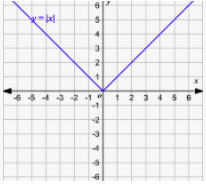
\includegraphics[scale=0.6]{pics/absvfunc.png}
	\newline \newline
	Anything with absolute value
	\newline \textbf{Format}: $y = |x|$
	
	\section{Square Root}
	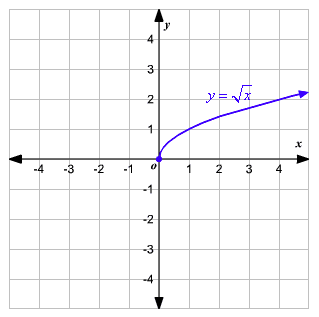
\includegraphics[scale=0.45]{pics/sqrtfunc.png}
	\newline \newline
	Anything with square root
	\newline \textbf{Format}: $y = \sqrt{x-a} + b$
	
	\section{Quadratic}
	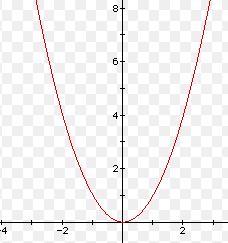
\includegraphics[scale=0.45]{pics/quadfunc.png}
	\newline \newline
	An equation creating a parabola
	\newline \textbf{Format}: $y = x^2 + bx + c$
	
	\section{Inverse}
	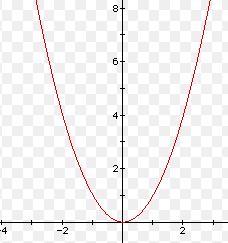
\includegraphics[scale=0.45]{pics/quadfunc.png}
	\newline \newline
	An function that is the opposite of another
	\newline \textbf{Format}: $y = x^2 + bx + c$
	
\end{document}